%%%%%%%%%%%%%%%%%%%%%%%%%%%%%%%%%%%%%%%%%
% Beamer Presentation
% LaTeX Template
% Version 1.0 (10/11/12)
%
% This template has been downloaded from:
% http://www.LaTeXTemplates.com
%
% License:
% CC BY-NC-SA 3.0 (http://creativecommons.org/licenses/by-nc-sa/3.0/)
%
%%%%%%%%%%%%%%%%%%%%%%%%%%%%%%%%%%%%%%%%%

%----------------------------------------------------------------------------------------
%	PACKAGES AND THEMES
%----------------------------------------------------------------------------------------
%!TEX encoding = UTF-8 Unicode


\documentclass[12pt,handout]{beamer}
\usepackage[utf8]{inputenc}
\usepackage[T1]{fontenc}
\usepackage{verbatim}

\mode<presentation> {

\usetheme{Pittsburgh}

}

\usepackage{graphicx} % Allows including images
\usepackage{booktabs} % Allows the use of \toprule, \midrule and \bottomrule in tables

%----------------------------------------------------------------------------------------
%	TITLE PAGE
%----------------------------------------------------------------------------------------

\title[]{Critical behaviour of the surface tension in the 3D Ising model} % The short title appears at the bottom of every slide, the full title is only on the title page

\author[]
{
Federico Belliardo \\
Marco Costa
} 

\institute[] % Your institution as it will appear on the bottom of every slide, may be shorthand to save space
{
Dipartimento di Fisica\\ % Your institution for the title page
Università di Pisa \\
\medskip
}
\date{\today} % Date, can be changed to a custom date

\begin{document}

\begin{frame}
\titlepage % Print the title page as the first slide
\end{frame}

%\begin{frame}
%\frametitle{Overview} % Table of contents slide, comment this block out to remove it
%\tableofcontents % Throughout your presentation, if you choose to use \section{} and \subsection{} commands, these will automatically be printed on this slide as an overview of your presentation
%\end{frame}

%----------------------------------------------------------------------------------------
%	PRESENTATION SLIDES
%----------------------------------------------------------------------------------------

\begin{frame}{Summary}

\begin{center}

\begin{itemize}
\item 3D Ising models
\item Definition of the surface tension
\item Cluster algorithm and boundary flip
\item (Notes on the implementation?)
\item Estimation of the errors and autocorrelation
\item Fit of the free energy
\item Fit of the critical behaviour
\item Conclusion
\end{itemize}

\end{center}
\end{frame}

\begin{frame}{3D Ising model}
\begin{center}
\begin{columns}
\begin{column}{0.43\textwidth}
 \[
\mathcal{H} = -\sum_{\langle x, y \rangle} J_{\langle x, y \rangle} s_x s_y
\]

\[
J_{\langle x, y \rangle} = 1\text{ ferromagnetic}
\]
\[
J_{\langle x, y \rangle} = -1\text{ antiferromagnetic}
\]
\end{column}
\begin{column}{0.57\textwidth}  %%<--- here
 \begin{figure}[!htb]
\centering
\includegraphics[scale=0.5]{ising3D.png}
\end{figure}
\end{column}
\end{columns}


\end{center}
\end{frame}

\begin{frame}{Definition of the surface tension}
\begin{center}


\begin{figure}[!htb]
\centering
\includegraphics[scale=0.5]{bound.png}
\end{figure}

\vspace{20pt}

{\Large
$
\sigma = -\lim_{L \rightarrow \infty} \frac{1}{L^2} \log \frac{Z_{+-}}{Z_{++}}$} $ \quad L \times L \times T,\, T = cL$

\note{L'ordine dei due limiti T e  non dovrebbe contare. Non so se si può "dimostrare" al nostro libello di rigore fisiamo T = 3L e facciamo il limite per L. Per sistemare la faccenda introduciamo una larghezza L del sistema e questa è l'unica lunghezza che va all'infinito.}

\note{$Z_{+-}$ e $Z_{++}$ sono le funzioni di partzione quando fisso cosa devono valere i layer di spin sul pavimento e sul soffito. Inserire piccola immagine per spiegarlo.}

\end{center}
\end{frame}

\begin{frame}
\begin{center}
\begin{figure}[!htb]
\centering
\includegraphics[scale=0.50]{comparison.png}
\end{figure}
\[
\sigma = -\lim_{L \rightarrow \infty} \frac{1}{L^2} \log \frac{Z_{+-}}{Z_{++}} = \lim_{L \rightarrow \infty} \frac{1}{L^2} \left( F_{+-} - F_{++} \right) = \lim_{L \rightarrow \infty} \frac{F_s}{L^2}
\]
\[\sigma = \text{interface free energy per unit area}\]

\note{Bisogna dire che nel limite termodinamico sopravvive una sola superficie di separazione.}

\end{center}
\end{frame}

\begin{frame}
\begin{center}

\begin{columns}
\begin{column}{0.50\textwidth}
\begin{center}
Redefinition of $Z_{++}$ and $Z_{+-}$.\\
\vspace{10pt}
$Z_{++} \rightarrow $ ferromagnetic link between \textbf{top and bottom}.\\
$Z_{+-} \rightarrow $ \textbf{anti}ferromagnetic link between \textbf{top and bottom}.\\
\vspace{10pt}
Always ferromagnetic link in $x$ and $y$.\\
\vspace{10pt}
Same definition for $\sigma$.\\
\vspace{10pt}
Periodic boundary conditions reduce the finite size effect.\\
\end{center}

\end{column}
\begin{column}{0.50\textwidth}  %%<--- here
\begin{figure}[!htb]
\centering
\includegraphics[scale=0.7]{antiferro.png}
\end{figure}
\end{column}
\end{columns}

\end{center}
\end{frame}

\begin{frame}
\begin{center}
{\Large Montecarlo simulations can't measure $Z$!\\}
\vspace{10pt}
Solution: $J_{\langle x, y \rangle}$ between top and bottom becomes a \textbf{dinamical variable} that is summed over in $Z$.\\
$J_{\langle x, y \rangle} = 1$ (periodic b.c.)\hspace{10pt}$J_{\langle x, y \rangle} = -1$ (antiperiodic b.c.)\\
Other $J_{\langle x, y \rangle}$ remains ferromagnetic.

\[
Z = \sum_{\lbrace s \rbrace, J} \exp \left( \beta \sum_{\langle x, y \rangle} J_{\langle x, y \rangle} s_x s_y \right)
\]

{\large \[
\frac{Z_{+-}}{Z_{++}} = \frac{\frac{Z_{+-}}{Z}}{\frac{Z_{++}}{Z}}=\frac{\langle \delta_{J = -1} \rangle}{\langle \delta_{J = + 1} \rangle}
\]}

Ratio of measurable expectation values.
\end{center}
\end{frame}

\begin{frame}
\begin{center}
We redefine the free energy of the interface in order to improve the convergence proprieties of $\frac{F_s}{L^2}$ to $\sigma$ when $L \rightarrow \infty$.
\vspace{10pt}
Thermodynamic limit {\Large $\rightarrow$} only \textbf{one} interface\\
\vspace{10pt}
For finite $L$ multiple interface can be present. An even number for $Z_{++}$ and odd for $Z_{+-}$.\\

\begin{figure}[!htb]
\centering
\includegraphics[scale=0.3]{multiple.png}
\end{figure}

\end{center}
\end{frame}

\begin{frame}
\begin{center}

$F_s$ is the free energy of a single surface. There are $\sim T$ different position for the interface.
\[Z_1 = T \exp \left( - F_s \right) = \exp \left( -F_S +\ln T \right) \]

\[ \frac{Z_{+-}}{Z_{++}} = \frac{Z_1 + \frac{Z_1^3}{3!} + \frac{Z_1^3}{5!} + ...}{1 +  \frac{Z_1^2}{2!} + \frac{Z_1^4}{4!} + ...} = \tanh \left( \exp \left( -F_S +\ln T \right) \right) \]

\[
F_S = \ln \left( T \right) - \ln \left( \frac{1}{2} \ln \left( \frac{1 + \frac{Z_{+-}}{Z_{++}}}{1 - \frac{Z_{+-}}{Z_{++}}} \right) \right) \quad \sigma = \lim_{L \rightarrow \infty} \frac{F_s}{L^2} \]


\end{center}
\end{frame}

\begin{frame}{Cluster algorithm and boundary flip}
\begin{center}

Cluster algorithms allow for simultaneous updates of large parts of the lattice. Thus reducing the autocorrelation time and the critical slowling down. Swendsen and Wang (1987).\\
\vspace{10pt}
Introduce link variables $\sigma_{\langle x, y \rangle} = \lbrace 0, 1 \rbrace$ on the lattice:
\begin{figure}[!htb]
\centering
\includegraphics[scale=0.4]{link.png}
\end{figure}

\note{Giustificare perché metto tre reticoli. Sono a diversa temperatura. A bassa T (alto beta) è facile formare i cluster. A basso beta è difficile.}

\end{center}
\end{frame}

\begin{frame}
\begin{center}

\[
Z = \sum_{\lbrace s \rbrace, J} \exp \left( \beta \sum_{\langle x, y \rangle} J_{\langle x, y \rangle} s_x s_y \right) = \sum_{\lbrace s \rbrace} \prod_{\langle x, y \rangle} \exp \left( \beta s_x s_y \right) 
\]


\end{center}
\end{frame}

%----------------------------------------------------------------------------------------

\end{document} 